% robust-ms-gate-v2.1.tex — REVTeX 4.2 port of docs/robust-ms-gate-manuscript-v2.1.md
% Compile: pdflatex; bibtex; pdflatex; pdflatex   (needs references.bib, figures/)
% DRAFT v2.1 — synced with the v2.1 markdown, which adds the SMOOTH GATE (AESE, Hughes25)
% as a second robustness axis: new contribution N6, Sec. II.E (adiabatic elimination),
% E7 (smooth x GBC combining map), Fig. 1 recast (two-axis, Fig1_toolchain_v2), new Fig. 6,
% new App. C, and refs Hughes25 / Sutherland16. Everything from v0.3 is preserved; the new
% material is this smooth-gate thread. Candidate revision — provided alongside the v0.3 .tex
% (docs/robust-ms-gate.tex) so the smooth-gate block can be accepted/rejected as a unit.
% Author block is a placeholder; finalize before submission.
\documentclass[aps,prapplied,twocolumn,superscriptaddress,floatfix,nofootinbib]{revtex4-2}
\usepackage{amsmath,amssymb}
\usepackage{graphicx}
\usepackage{bm}
\graphicspath{{figures/}}
% discourage bad hyphenation of code/compound terms
\hyphenation{gener-ator com-pen-sa-tion Lamb-Dicke wave-form}

\begin{document}

\title{Analytic design and open-system verification of robust M\o lmer--S\o rensen
gates: quantifying the coherent--incoherent trade-off}

\author{Siridech B.}
\email{siridech.bo@kmitl.ac.th}
\affiliation{King Mongkut's Institute of Technology Ladkrabang (KMITL), Bangkok, Thailand}
% Placeholder author block — finalize before submission.

\begin{abstract}
Robust M\o lmer--S\o rensen (MS) gates are designed almost exclusively against
\emph{coherent} error, while the \emph{incoherent} environment (motional heating,
dephasing, spontaneous emission during the gate) is treated separately. Because the
leading robust-control techniques necessarily extend the gate~time, coherent-error
suppression is bought at the price of increased incoherent accumulation. We present a
cross-validated toolchain that couples a fast \emph{analytic} MS designer/verifier
(second-order Magnus in the commuting $\sigma_x$ basis, $O(M)$ per gate for $M$ modes)
to a \emph{full open-system} Lindblad integrator carrying the same parameters. We
(i)~confirm the two engines agree to $\sim\!3\times10^{-9}$ in Bell-state infidelity in
the closed-system limit; (ii)~reproduce the coherent robustness of the symmetric-robust
($2.5\times10^{3}\times$ suppression of the symmetric-drift residual) and generator-based
compensation (GBC, $\varepsilon^2\!\to\!\varepsilon^4$ with $\varepsilon\equiv\Delta\omega\tau$)
schemes; and (iii)~map the coherent--incoherent trade-off: GBC's $\varepsilon^4$ advantage
costs a $\approx\!4\times$ gate~time (hence $\approx\!4\times$ incoherent error), so a
crossover asymmetric detuning $\Delta\omega^\times\!\propto\!\sqrt{I_{\rm incoh}}$ separates
a regime where the single robust gate wins from one where GBC wins. Concretely, for a
center-of-mass mode at $\omega_z=2\pi\times1$~MHz driven at $\delta=2\pi\times50$~kHz
($\tau\approx20~\mu$s) with heating $\dot{\bar n}\approx1$~phonon/ms, the crossover lies at
$\Delta\omega^\times\approx2\pi\times2.7$~kHz. We further show that (iv)~the useful
compensation \emph{depth} is shallow --- recursive GBC plateaus at $\varepsilon^4$, so the
optimum is $k^\star\!\in\!\{0,1\}$ (one GBC or none); and (v)~the trade-off is robust to the
real system --- species-independent (${}^{40}$Ca$^+\!\equiv\!{}^{171}$Yb$^+$-Raman in
dimensionless units), shifted by $\lesssim\!10\%$ under spectator-mode load (the incoherent
sensitivity is target-mode dominated), and consistent with a full non-RWA + beyond-Lamb-Dicke
model ($\lesssim\!10^{-4}$ residual at the ${}^{40}$Ca$^+$ operating point). Finally,
(vi)~we bring the recent \emph{smooth gate} (adiabatic elimination of spin--motion entanglement,
AESE~\cite{Hughes25}) into the same open-system framework as a second, orthogonal robustness axis:
AESE crushes the symmetric (motional/temperature) axis (spin--motion residual suppressed
$\sim\!800\times$, motional-noise filter $\sim\!10^{6}\times$ below the diabatic gate) while GBC
crushes the asymmetric axis, so their infidelities add. Because the smooth gate is intrinsically
long ($\tau_{\rm smooth}\!\approx\!14\tau$), it is symmetric-robust but asymmetric-fragile; a
four-scheme (plain/smooth/GBC/smooth+GBC) decision map shows smooth+GBC wins only where both error
axes are large, with an add-GBC-to-smooth threshold $\Delta\omega^\times\!\approx\!3.5\times10^{-3}$.
\end{abstract}

\maketitle

\section{Introduction}
Trapped ions are among the leading platforms for quantum computation, with two-qubit MS
fidelities above $99.9\%$~\cite{Ballance16,Gaebler16,Clark21}. Coherent control error
splits, following the red/blue-tone geometry of the bichromatic drive, into a
\emph{symmetric} error (both sidebands shift together, a motional-detuning drift, an
unclosed phase-space trajectory) and an \emph{asymmetric} error (the tones shift
oppositely, a drift of the qubit center line, a $\sigma_z$ rotation on both qubits). The
former is suppressed by robust waveforms~\cite{Leung18,Milne20,Roos08,Zhu06} and, most recently,
by the \emph{smooth gate}~\cite{Hughes25}, which ramps the sideband detuning adiabatically so the
spin-dependent displacement returns to the origin regardless of a slow motional-frequency drift
(adiabatic elimination of spin--motion entanglement); the latter
does not commute with the entangler $G=\sigma_x^{j_1}\sigma_x^{j_2}$ and was recently
addressed by generator-based compensation (GBC), which cancels the residual $\sigma_z$ to
first order at the cost of a doubled-gate-time segment. For ${}^{40}$Ca$^+$, asymmetric
error is the second-largest error source~\cite{Pogorelov21,Postler22}.

All of this is validated in the closed-system limit, yet every robustness technique
\emph{lengthens the gate}, and longer gates accumulate more incoherent error. We ask:
\emph{how much of the coherent robustness survives realistic dissipation, and where is
the net-fidelity optimum?} Answering it requires one framework that both designs the
robust coherent pulse and verifies it under the full master equation.

\paragraph*{Relation to prior work.} The analytic core we use --- second-order Magnus in
the $\sigma_x$ basis, phase-space closure, the amplitude-modulation waveform solver, and
the GBC construction --- is established: the Sorensen--M\o lmer and frequency-modulation
results are from Refs.~\cite{Sorensen00,Leung18}, and the symmetric/asymmetric-robust
waveform and GBC construction were recently developed by an \emph{independent group},
Zhang \emph{et~al.}~\cite{Zhang25}, whose coherent-error results we reproduce as validation
baselines (Sec.~\ref{sec:val}, Fig.~\ref{fig:val}) and build upon. The \emph{smooth gate} we compare
and combine with GBC is that of Hughes \emph{et~al.}~\cite{Hughes25}, likewise an independent group;
we reproduce its motional-robustness signatures (Sec.~\ref{sec:smooth}, E7) and use it as
the second robustness axis. We claim no novelty for that coherent machinery, nor for either robust
construction --- only for their open-system comparison and combining. Our contributions are on the
open-system and trade-off side:
(N1)~a unified, cross-validated design$\to$open-system-verify pipeline (analytic
$\leftrightarrow$ numerical agreement $\sim\!3\times10^{-9}$); (N2)~the quantitative
coherent--incoherent trade-off map and its crossover law
$\Delta\omega^\times\!\propto\!\sqrt{I_{\rm incoh}}$; (N3)~the optimal-depth result
(recursive GBC plateaus at $\varepsilon^4$, so $k^\star\!\in\!\{0,1\}$); (N4)~the extension
to $N\!\le\!4$-ion chains with Coulomb-equilibrium mode spectra, with the finding that the
incoherent sensitivity is \emph{target-mode dominated}; (N5)~the species-independence of
the trade-off and a non-RWA + beyond-Lamb-Dicke bound certifying the RWA+LD model; and
(N6)~the integration of the \emph{smooth gate} (AESE~\cite{Hughes25}) as a second, orthogonal
robustness axis, with the resulting smooth$\times$GBC combining map --- a four-scheme decision
boundary with an add-GBC threshold $\Delta\omega^\times\!\approx\!3.5\times10^{-3}$ (E7),
showing where two robust-control techniques should be \emph{combined} rather than chosen between.

\section{Theoretical framework}
\subsection{Ideal multi-mode MS Hamiltonian}
In the Lamb--Dicke and rotating-wave approximations,
\begin{equation}
\hat H_{\rm int}(t)=\tfrac12\Omega(t)\sum_{j,m}\eta_m b^m_j\,\sigma_x^j
\big(a_m^\dagger e^{i\delta_m t}+a_m e^{-i\delta_m t}\big).
\end{equation}
Here $\Omega(t)$ is the single-beam carrier Rabi frequency --- so the per-ion sideband coupling is
$\eta_m b^m_j\Omega/2$, the $\tfrac12$ being the usual carrier factor (each of the two bichromatic
tones drives one sideband) --- $\eta_m$ the mode-$m$ Lamb--Dicke parameter, $b^m_j$ its eigenvector
amplitude on ion $j$, and $\delta_m$ the drive detuning. The coupling operators all commute, so the
second-order Magnus expansion terminates:
\begin{equation}
\hat U(\tau)=\exp\!\Big[i\Theta\,\sigma_x^{j_1}\sigma_x^{j_2}
-\tfrac{i}{2}\!\sum_{j,m}(\alpha_m a_m^\dagger+\alpha_m^* a_m)\eta_m b^m_j\sigma_x^j\Big],
\end{equation}
\begin{equation}
\begin{aligned}
\alpha_m(\tau)&=\int_0^\tau\!\Omega(t)\,e^{i\delta_m t}\,dt,\\
\Theta&=\tfrac12\sum_m\eta_m^2 b^m_{j_1}b^m_{j_2}\!\iint\!\Omega\Omega\,\sin[\delta_m(t_1{-}t_2)].
\end{aligned}
\end{equation}
The gate is clean when $\alpha_m(\tau)=0$ and $\Theta=\pi/4$. Because the $\sigma_x^j$ commute,
this multi-mode phase is \emph{exact}, not a cross-term-truncated approximation --- a point we
verify against the full integrator in E5.
\emph{Convention:} we write the entangler on the pairwise operator $\sigma_x^{j_1}\sigma_x^{j_2}$
(maximally entangling at $\Theta=\pi/4$); the equivalent collective form $\exp(i\Theta_S S_x^2)$,
$S_x{=}\sum_j\sigma_x^j$, has $S_x^2{=}2\mathbb I{+}2\sigma_x^{j_1}\sigma_x^{j_2}$ (spectrum
$\{4,0,0,4\}$), so the \emph{same} gate is $\Theta_S{=}\Theta/2{=}\pi/8$. The shaped-pulse engine
reports the $S_x^2$ value, so waveform-level results (e.g.\ Table~\ref{tab:e6}) quote $\pi/8$ while
the GBC/theory sections quote the pairwise $\pi/4$ --- the identical gate.

\subsection{Coherent errors and robust waveform}
During the gate the spin-dependent force drives each motional mode around a loop in phase
space; $\alpha_m(t)$ is its spin-dependent displacement and the enclosed area is $\Theta$. Two
conditions must hold at $\tau$: every loop must \emph{close} ($\alpha_m(\tau)=0$), or the qubits
stay entangled with the motion and dephase; and closure must survive \emph{slow drift} of the
mode frequency (the symmetric error). A common-mode asymmetric error separately adds
$\tfrac{\Delta\omega}{2}\sum_j\sigma_z^j$. Imposing a symmetric pulse $\Omega(t)=\Omega(\tau-t)$
and zero time-averaged displacement $\int_0^\tau\alpha_m\,dt=0$ achieves both robustness goals
at once: the time-reversal symmetry makes the trajectory palindromic, forcing
$\partial_{\delta_m}\alpha_m(\tau)=0$ so the loop reopens only at \emph{second} order in a
frequency drift (passive suppression of quasi-static motional noise), while
$\int\alpha_m\,dt=0$ ($\beta_m(\tau)=0$) removes the residual cross term coupling the center-line
error to leftover motion. With every mode closed and $\beta_m=0$ the operator collapses to the
motion-free form
\begin{equation}
\hat U(\tau)=\exp\!\Big[i\Theta\,\sigma_x^{j_1}\sigma_x^{j_2}-\tfrac{i}{2}\Delta\omega\tau\!\sum_j\sigma_z^j\Big].
\label{eq:star}
\end{equation}
Equation~\eqref{eq:star} is the linchpin of the analysis: the motion factors out (a spectator),
so the coherent gate is the ideal entangler plus a residual common-$\sigma_z$ set by the
center-line error, and \emph{all} coherent-error questions reduce from
$2^N\!\times\!\prod_m\mathcal F_m$ to the $4\times4$ two-qubit space --- the collapse that makes
the design/verification analytic at $O(1)$ cost (and the two engines cross-validate to
$\sim\!10^{-9}$, Sec.~\ref{sec:val}). The piecewise-constant waveform solves $A\mathbf{x}=\mathbf 0$
(closure, \emph{linear} in the amplitudes) and $\mathbf{x}^{\mathsf T}M\mathbf{x}=\Xi$ (angle,
\emph{quadratic}), giving the minimum-intensity solution
$\mathbf{x}=\sqrt{\Xi/\lambda}\,\ker(A)\mathbf v_\lambda$~\cite{Zhang25,Leung18}. Since $\Theta$ is
a quadratic form, its \emph{sign} is fixed by the mode geometry (loop orientation) and cannot be
set by rescaling $\Omega$; the solver returns the requested sign when the nullspace admits it and
otherwise the conjugate gate (a single-qubit $Z$ apart), reporting which.

\subsection{Generator-based compensation}
Not every error can be refocused: a trailing single-qubit rotation removes any error commuting
with the entangler, but the center-line error is a common $\sigma_z$, $\hat E=\tfrac12\sum_j\sigma_z^j$,
that \emph{anticommutes} with $G=\sigma_x\sigma_x$ ($\{\hat G,\hat E\}=0$) and so cannot be commuted
through and undone locally --- it is bound into the two-qubit evolution, and is the leading
\emph{coherent} residual once the motional errors are shaped away~\cite{Pogorelov21,Postler22}.
GBC realizes the first-order-exact three-gate sequence
$\hat U^{\rm gbc}_\varepsilon=\hat U_\varepsilon\hat U^\dagger_{2\varepsilon}\hat U_\varepsilon
=\hat U_{\rm ideal}+o(\varepsilon^2)$, with $\hat U^\dagger_{2\varepsilon}=\hat\Pi\,\hat
U_{2\varepsilon}(-\Theta)\,\hat\Pi$, $\hat\Pi=\sigma_x\!\otimes\!\sigma_x$, and
$\varepsilon\equiv\Delta\omega\tau$. It works because $\hat\Pi\hat G\hat\Pi=+\hat G$ but
$\hat\Pi\hat E\hat\Pi=-\hat E$: conjugation by $\hat\Pi$ preserves the entangler while flipping
the sign of the error, so the sequence is a spin echo \emph{on the center-line error that leaves
the entangling action intact} --- the outer legs accrue $+\Theta,+\varepsilon$; the middle leg,
conjugated and run for $2\tau$, accrues $-\Theta$ entangling but $-2\varepsilon$ error, so the
first-order error cancels ($\varepsilon-2\varepsilon+\varepsilon=0$) while the phases sum to the
target. The residual infidelity is thus $O(\varepsilon^4)$ (GBC) vs $O(\varepsilon^2)$
(uncompensated), a $10^2$--$10^4\times$ suppression (App.~\ref{app:eps}). GBC is
\emph{generator-based} --- it needs only $\{\hat G,\hat E\}=0$ and Eq.~\eqref{eq:star}, not the
microscopic pulse, so it composes with any robust waveform --- and, because Eq.~\eqref{eq:star}
is motion-free, it lives entirely in the $4\times4$ space (no Fock integration; Sec.~V, U2). Its
price is the $4\tau$ duration ($\tau+2\tau+\tau$), hence $\approx4\times$ incoherent error: the
$\varepsilon^4$-coherent-gain / $4\times$-incoherent-cost tension is the trade-off we quantify.
Nesting does not help beyond one level (E4).

\subsection{Open-system model (this work)}
Everything above --- mode closure, robust shaping, GBC --- is a \emph{coherent} design:
it optimizes a unitary while treating the environment as absent. This subsection restores the
environment, and is the crux of the paper. The motivation is the tension built into the
preceding sections: robustness is bought with \emph{gate time} (a multi-segment waveform, and
GBC's $4\tau$), and a longer gate sits longer in contact with the bath, so whether a
coherent-robust gate is truly more faithful cannot be settled by any coherent theory --- it
requires evolving the \emph{same} pulse sequence under the full master equation. We do exactly
that: $\rho$ on $\mathbb C^{2^N}\!\otimes\!\prod_m\mathcal F_m$ evolves under
\begin{equation}
\dot\rho=-i[\hat H(t),\rho]+\sum_c\big(L_c\rho L_c^\dagger-\tfrac12\{L_c^\dagger L_c,\rho\}\big),
\end{equation}
with $\hat H(t)$ the \emph{shaped} Hamiltonian of Sec.~II (including the $\Delta\omega\,\sigma_z$
center-line term, so the integrator sees the identical designed waveform), and collapse operators
$L_{\rm heat}^{-}=\sqrt{\kappa(\bar n{+}1)}\,a_m$, $L_{\rm heat}^{+}=\sqrt{\kappa\bar n}\,a_m^\dagger$
(anomalous motional heating from electrode field noise --- the dominant motional decoherence,
$\dot{\bar n}=\kappa\bar n$, and the channel the gate-time growth most exposes since the gate
mechanism \emph{is} spin--motion coupling), $L_\phi^{j}=\sqrt{\gamma_\phi/2}\,\sigma_z^{j}$ (qubit
dephasing from magnetic-field/laser-phase noise, $T_2{=}2/\gamma_\phi$), and
$L_{\rm se}^{j}=\sqrt{\Gamma}\,\sigma_-^{j}$ (off-resonant scattering during the drive). All three
are set by directly measured lab quantities ($\dot{\bar n}$, $T_2$, $\Gamma$), not fit constants.
Evolving a coherent-optimized robust pulse under the complete CPTP master equation --- no secular
approximation, no adiabatic elimination --- is the layer the robust-control literature omits and
our verifier supplies (N1): it turns ``how robust is the \emph{unitary}?'' into ``how faithful is
the \emph{gate}?'', and makes the trade-off of Sec.~VI a measurement rather than an assumption.

\subsection{Adiabatic elimination of spin--motion entanglement (the smooth gate)}\label{sec:smooth}
The robust waveform (Sec.~II\,B) and GBC (Sec.~II\,C) suppress the two coherent error axes by
shaping and by an echo sequence, respectively. A structurally different route to the
\emph{symmetric} axis is the smooth gate of Hughes \emph{et~al.}~\cite{Hughes25}: hold the drive
envelope $\Omega$ essentially constant and instead ramp the detuning $\delta(t)$ \emph{slowly}, so
the spin-dependent displacement is eliminated \emph{adiabatically} rather than by a designed
closure. In the forced ($\pm$) spin sector, $\hat H=\delta(t)a^\dagger a+\Omega(t)(a+a^\dagger)$
and the displacement $\alpha(t)=\langle a\rangle$ obeys the driven-oscillator equation
\begin{equation}
\dot\alpha=-i\big(\delta(t)\,\alpha+\Omega(t)\big),\qquad \dot\theta_g=\Omega(t)^2/\delta(t),
\label{eq:aese}
\end{equation}
with the entangling phase $\theta_g=\int_0^\tau\Omega^2/\delta\,dt$~\cite{Hughes25}. A clean gate
needs $\alpha(\tau)=0$ at the target $\theta_g$. Two limits close the loop: \emph{diabatic} (DESE,
$\delta$ constant, $\Omega$ ramped fast) --- the standard MS gate, resonant so a static drift
$\delta\!\to\!\delta+\Delta\delta$ reopens the loop at first order; and \emph{adiabatic} (AESE,
$\Omega$ constant, $\delta(t)$ swept slowly $\delta_{\max}\!\to\!\delta_{\min}\!\to\!\delta_{\max}$
via $\delta(s)=(b+c\,g(s))^{-1/j}$, \cite{Hughes25} Eq.~(18)) --- here $\alpha$ tracks its
instantaneous equilibrium $-\Omega/\delta(t)$ and is returned to the origin by $\Omega\!\to\!0$ at
the ends \emph{independently} of $\Delta\delta$, the source of the motional robustness. The module
\textsf{ion-smooth} integrates Eq.~\eqref{eq:aese} with the classical trajectory (no Fock space),
exact for the coherent diagnostics: the static-drift residual $|\alpha(\tau)|$ and the filter
function $F(\omega)=\langle|\alpha(\tau)|^2\rangle_\varphi/\varepsilon^2$ for an oscillatory
mode-frequency noise (\cite{Hughes25} App.~B). AESE acts \emph{only} on the symmetric axis (it does
nothing to the center-line $\sigma_z$), so it is orthogonal and complementary to GBC --- their
leading infidelities add. But the adiabatic sweep makes the gate \emph{long}
($\tau_{\rm smooth}\!\approx\!14\tau$ at the parameters of E7), and since the
center-line error enters as $\varepsilon=\Delta\omega\tau$, the smooth gate is \emph{more} exposed to
the asymmetric axis than a short gate --- exactly the case where appending GBC pays (E7).

\section{Toolchain}
\begin{figure}[t]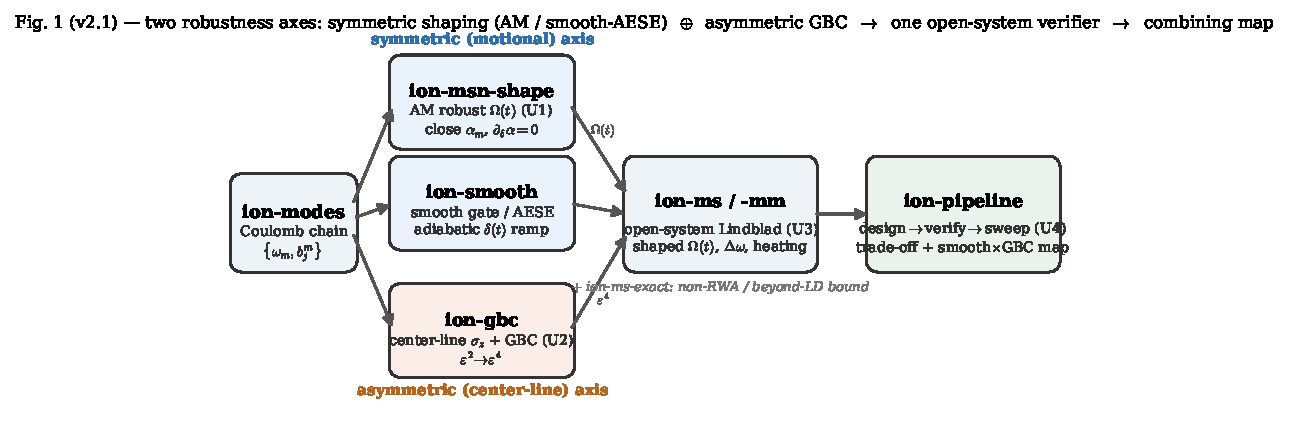
\includegraphics[width=\columnwidth]{Fig1_toolchain_v2}
\caption{The design$\to$verify$\to$sweep toolchain, organized by \emph{robustness axis}. The
chain-mode solver feeds two orthogonal coherent-robustness families --- the symmetric (motional)
axis (\textsf{ion-msn-shape}, AM robust waveform; \textsf{ion-smooth}, adiabatic AESE gate) and the
asymmetric (center-line) axis (\textsf{ion-gbc}, GBC $\varepsilon^2\!\to\!\varepsilon^4$) --- both
feeding a single open-system Lindblad verifier (\textsf{ion-ms}/\textsf{ion-ms-mm}, with
\textsf{ion-ms-exact} the non-RWA/beyond-LD bound) and then the sweep driver (\textsf{ion-pipeline})
that produces the trade-off and smooth$\times$GBC combining maps. Upgrade tags U1--U4 as in the
text.}\label{fig:toolchain}\end{figure}
The toolchain follows one philosophy --- \emph{design cheaply, verify honestly, sweep to map}
--- with two independent engines carrying the same physical parameters (Fig.~\ref{fig:toolchain}).
All modules are framework-free JavaScript, node-importable and browser-runnable, each covered by
a \textsf{node:assert} suite and sharing one flat interleaved-complex RK4 core, so every number
below regenerates from the released code with no build step.

\emph{(A) Analytic designer/verifier} --- \textsf{ion-msn(-shape)}: in the commuting-$\sigma_x$
basis where the Magnus series terminates, it evaluates $\Theta$, the displacements $\alpha_m$ and
their closure residuals, and the Bell fidelity as the geometric phase times the thermal
decoherence factor $C_{ij}=\exp[-\sum_m(2\bar n_m{+}1)|\Delta\alpha_m|^2/2]$ (so an unclosed loop
is penalized), and solves the robust waveform of Sec.~II. Cost $O(M)$, no Fock tensor ---
milliseconds for a full chain. \emph{(B) Open-system verifiers} --- \textsf{ion-ms} integrates
the $4N_{\rm Fock}$ single-mode density matrix under the full master equation, kept CPTP by an
adaptive RK4 sub-step bounded per segment by the fastest active scale
$\max(\Omega_0,\delta_m,|\omega_z{-}\delta|,\kappa,\gamma_\phi)$ plus a per-step Hermitization, with
$\mathrm{Tr}\,\rho{=}1$ and $\rho\succeq0$ asserted as invariants even with all noise on (the
numerical rigor the open-system results depend on); \textsf{ion-ms-mm} generalizes to $M$ modes
(dimension $4\prod_m N_{\rm Fock}^{(m)}$) with the Hermiticity identity $\rho H=(H\rho)^\dagger$
making each product sparse-first, $O(\dim^2 M)$ not $O(\dim^3)$; \textsf{ion-ms-exact} is a
statevector reference keeping the full $\sin[\eta(a{+}a^\dagger)]$ and lab-frame $\omega_z
a^\dagger a$ (no LD, no vibrational RWA). \emph{(C) Chain modes} --- \textsf{ion-modes}: Coulomb
equilibrium by Newton iteration and axial modes from the James Hessian; the eigenvectors $b^m_j$
feed the per-ion couplings $\eta_m b^m_j$ that (A) and (B) share, so both see the same real chain.
\emph{(D) Compensation, driver, comparators} --- \textsf{ion-gbc} (the $4\times4$
asymmetric-error/GBC gate, recursively nestable), \textsf{ion-pipeline} (the design$\to$verify$\to$noise-scan
driver), \textsf{ion-ms-pm} (phase-modulated comparator, E6), \textsf{ion-jitter} (timing-jitter
model), and \textsf{ion-smooth} (the smooth gate / AESE of Sec.~\ref{sec:smooth}: integrates the
semiclassical $\alpha(t)$ under a ramped $\delta(t)$, returning the static-drift residual and filter
function, and drives the four-scheme combining map of E7). \emph{(E) Cross-validation}: analytic and numerical Bell fidelities agree to
$|\Delta F|\approx3\times10^{-9}$ (closed system), and the multi-mode integrator reproduces the
analytic two-ion kernel to $10^{-6}$ (E5) --- a common ground truth fixed \emph{before} dissipation
is switched on, which is what lets us attribute the open-system results to the incoherent layer
alone.

\section{Validation}\label{sec:val}
\begin{figure}[t]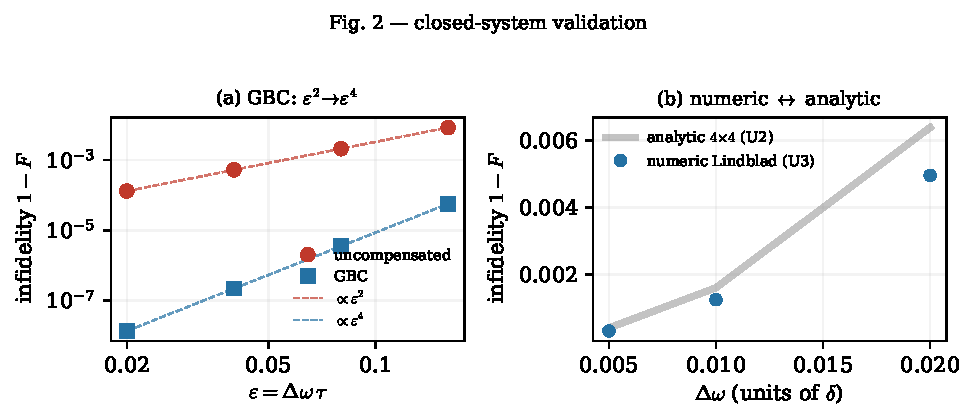
\includegraphics[width=\columnwidth]{Fig2_validation}
\caption{Closed-system validation. (a)~GBC turns the $\varepsilon^2$ asymmetric-error
infidelity ($1-F$ vs $\varepsilon=\Delta\omega\tau$) into $\varepsilon^4$ (measured ratios
$4.00$/$15.97$ per doubling of $\varepsilon$). (b)~The numerical Lindblad gate (U3) and the
analytic $4\times4$ gate (U2) agree on the $\Delta\omega$-error infidelity, scaling
$\propto\Delta\omega^2$.}\label{fig:val}\end{figure}
We validate the coherent physics two independent ways before adding dissipation --- internally, by
cross-checking the two engines, and externally, against Zhang \emph{et al.}~\cite{Zhang25} --- since
the trade-off study rests on attributing any open-system infidelity to the dissipative layer, which
is credible only if the coherent core is first proven correct.

\emph{B1 (engine agreement).} The analytic designer and the Lindblad integrator share nothing but the
physical parameters --- one is a Fock-free second-order Magnus evaluation in the $\sigma_x$ basis, the
other a full density-matrix RK4 in truncated Fock space, effectively two different theories of the
same gate --- yet their Bell fidelities agree to $|\Delta F|\approx3\times10^{-9}$ across three
physically distinct regimes (closed loop, deliberate phase error, unclosed loop) and for both
constant and shaped drives. This is stringent: it demands that both capture the geometric phase, the
per-mode closure, and the thermal overlap identically. The check extends to the multi-mode integrator,
which reproduces the analytic two-ion kernel to $10^{-6}$ and a three-ion chain to $4.6\times10^{-4}$
(E5), so it is not an artifact of the single-mode case.

\emph{B2 (reproduces \cite{Zhang25}).} The App-C robust waveform suppresses the symmetric-drift
closure residual by $2.5\times10^{3}$ with quadratic (vs.\ linear) scaling --- the signature of
first-order $\partial_\delta\alpha=0$ insensitivity --- and the asymmetric-error infidelity scales as
$\varepsilon^2$ uncompensated (measured ratio $4.00$ per doubling) vs.\ $\varepsilon^4$ with GBC
(ratio $15.97$), reproducing their Fig.~5 (Fig.~\ref{fig:val}a); the composed three-gate unitary is
unitary to $10^{-16}$. Together, B1 and B2 fix a common ground truth: any fidelity change reported
below is a property of the open-system model, not of the coherent core or either engine.

\section{Numerical experiments}
Single-mode MS gate unless stated, $\eta=0.1$ (${}^{40}$Ca$^+$; $\nu_z=1$~MHz
$\Rightarrow\eta\approx0.097$, matching~\cite{Zhang25}), $\delta\equiv1$ (frequency unit),
$K=1$, $N_{\rm Fock}=18$. The incoherent floor is Fock-converged: the single-gate infidelity
under heating is identical to five significant figures across $N_{\rm Fock}=12$--$28$ at every
rate tested (e.g. $8.231\times10^{-2}$ at $\kappa=0.02$; $1.727\times10^{-1}$ at $\kappa=0.05$).

\textit{Method (validated-component decomposition).} GBC reaches $\varepsilon^4$ only when
$\beta_m=0$ (robust waveform); a constant single-mode drive has $\int\alpha\,dt\neq0$, so a
constant-leg GBC cancels only to $\varepsilon^2$ (verified $N_{\rm Fock}$-independently: identical
at $N_{\rm Fock}=18,30$). We therefore take GBC's coherent part from the analytic gate
($\varepsilon^4$) and its incoherent part from the numerically integrated $4\tau$ sequence at
$\Delta\omega=0$, combined additively. This is leading-order exact: the GBC time is
\emph{exactly} $4\tau$ ($\tau{+}2\tau{+}\tau$, the ``$\approx$'' flagging only fast global-$\Pi$
single-qubit pulses), and the cross-term is $O(\varepsilon^4\!\cdot\!\kappa\tau)$ --- negligible
against either channel.

\paragraph{E1 --- incoherent baseline.} With no coherent error, GBC's infidelity is purely its
incoherent cost, and it is a clean $\approx4\times$ the single gate across heating rates
(Fig.~\ref{fig:e1}), its $4\tau$ vs $\tau$ cost. The penalty is real and dominant --- the price
\emph{any} gate-lengthening scheme must pay, and the reason a trade-off exists at all --- and its
rate-independence validates the additive decomposition: the incoherent error tracks gate time
linearly, so the two floors stay in fixed $4{:}1$ proportion regardless of the heating magnitude.

\paragraph{E2 --- trade-off curve.} At fixed noise the single gate rises $\propto\Delta\omega^2$
(uncompensated coherent error) while GBC stays flat at its $4\times$ incoherent floor (its
$\varepsilon^4$ term negligible); the two \emph{cross} at $\Delta\omega^\times$
(Fig.~\ref{fig:e2}). This rising-vs-flat crossing is the signature of the result: GBC buys
immunity to center-line drift for a fixed incoherent surcharge, and wins only once the drift is
large enough to push the single gate above that surcharge --- $\Delta\omega^\times$ is where the
experimentalist's choice flips.

\paragraph{E3 --- trade-off map.} Sweeping the noise floor turns E2 into a decision boundary:
$\Delta\omega^\times$ grows monotonically with the incoherent floor (Table~\ref{tab:e3},
Fig.~\ref{fig:e3}), scaling as $\sqrt{I_{\rm incoh}}$ since equating the single gate's coherent
error to GBC's extra $3\tau$ incoherent cost gives $\varepsilon^2(\Delta\omega^\times)\!\sim\!3I_{\rm incoh}$.
The practical reading: the crossover tracks the trap and does so gently ($4\times$ lower noise
lowers it only $2\times$), so a quieter trap makes GBC pay off sooner.
Repeating for ${}^{40}$Ca$^+$ ($\eta=0.10$) and ${}^{171}$Yb$^+$-Raman ($\eta=0.19$) gives
\emph{identical} crossovers; only the drive differs ($\Omega_{\rm closure}=5.0$ vs $2.6$,
$\propto1/\eta$), because $\eta\Omega=\delta/(2\sqrt K)$ is fixed at closure.

\paragraph*{Physical units.} With $\delta\equiv1$ as the frequency unit, a concrete map:
a center-of-mass mode at $\omega_z=2\pi\times1$~MHz driven at $\delta=2\pi\times50$~kHz gives a
single-gate time $\tau=2\pi/\delta\approx20~\mu$s. A heating rate $\dot{\bar n}\approx1$~phonon/ms
corresponds to $\kappa\approx3\times10^{-3}$ ($\kappa=\dot{\bar n}/\delta$), the fourth row of
Table~\ref{tab:e3}, where $\Delta\omega^\times\approx0.055$ translates to a physical center-line
tolerance $\Delta\omega^\times\approx2\pi\times2.7$~kHz: below it, run the single robust gate;
above it, GBC pays off.

\begin{figure}[t]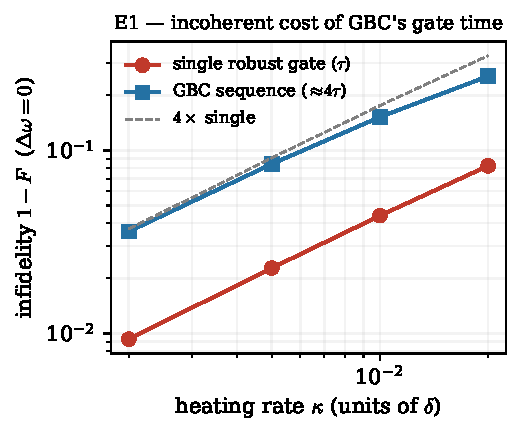
\includegraphics[width=0.86\columnwidth]{Fig3_E1_incoherent}
\caption{E1: GBC's $\approx4\tau$ incoherent infidelity ($1-F$) vs heating rate $\kappa$
(units of $\delta$), $\approx4\times$ the single gate throughout.}\label{fig:e1}\end{figure}
\begin{figure}[t]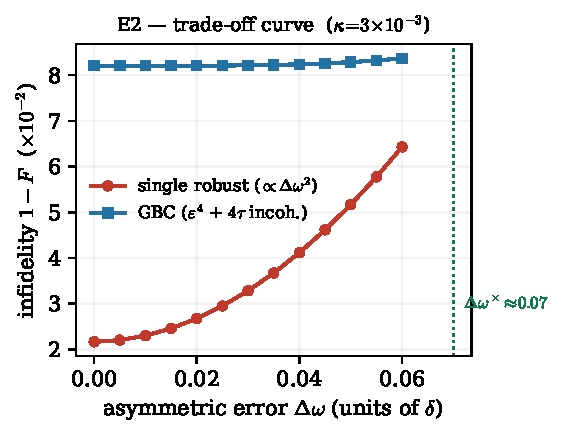
\includegraphics[width=0.86\columnwidth]{Fig4_E2_tradeoff}
\caption{E2: single-gate ($\propto\Delta\omega^2$) and GBC ($\approx$ flat) infidelities vs
asymmetric detuning $\Delta\omega$ (units of $\delta$); they cross at
$\Delta\omega^\times$.}\label{fig:e2}\end{figure}
\begin{figure}[t]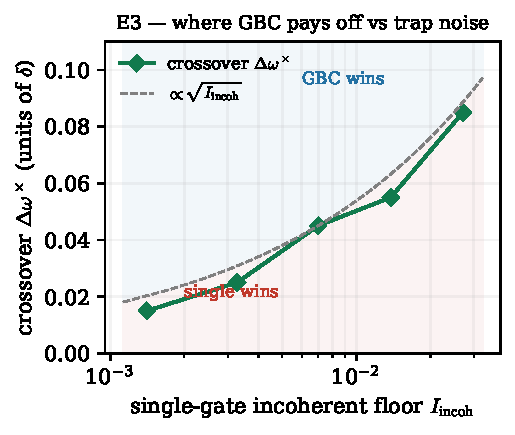
\includegraphics[width=0.86\columnwidth]{Fig5_E3_crossover}
\caption{E3: crossover $\Delta\omega^\times$ (units of $\delta$) vs incoherent floor
$I_{\rm incoh}$, scaling as $\sqrt{I}$; single-gate-wins and GBC-wins regions shaded. For the
reference $\delta=2\pi\times50$~kHz, the $\Delta\omega^\times$ axis spans
$\sim\!2\pi\times(0.7$--$4)$~kHz.}\label{fig:e3}\end{figure}

\begin{table}[t]\caption{E3 crossover vs heating $\kappa$ ($\bar n_{\rm th}=1$). Rightmost
column gives the physical $\Delta\omega^\times$ for the reference $\delta=2\pi\times50$~kHz.}
\label{tab:e3}
\begin{ruledtabular}\begin{tabular}{ccccc}
$\kappa$ & single incoh. & GBC incoh. & $\Delta\omega^\times$ & $\Delta\omega^\times/2\pi$ (kHz)\\ \hline
$3\times10^{-4}$ & $1.4\times10^{-3}$ & $5.6\times10^{-3}$ & $0.015$ & $0.75$\\
$7\times10^{-4}$ & $3.3\times10^{-3}$ & $1.3\times10^{-2}$ & $0.025$ & $1.25$\\
$1.5\times10^{-3}$ & $7.0\times10^{-3}$ & $2.7\times10^{-2}$ & $0.045$ & $2.25$\\
$3\times10^{-3}$ & $1.4\times10^{-2}$ & $5.3\times10^{-2}$ & $0.055$ & $2.75$\\
$6\times10^{-3}$ & $2.7\times10^{-2}$ & $9.9\times10^{-2}$ & $0.085$ & $4.25$\\
\end{tabular}\end{ruledtabular}\end{table}

\paragraph{E4 --- optimal robustness depth.} We nest GBC via its physical
error-flip, $\hat U^{(k)}_\varepsilon=\hat U^{(k-1)}_\varepsilon[\hat\Pi\hat
U^{(k-1)}_{2\varepsilon}(-\Theta)\hat\Pi]\hat U^{(k-1)}_\varepsilon$, so the gate time grows
as $4^k\tau$. The coherent infidelity does \emph{not} keep improving: it drops
$\varepsilon^2\!\to\!\varepsilon^4$ from $k{=}0\!\to\!1$ then \emph{plateaus} at $\varepsilon^4$
for all $k\ge1$ (measured exponents $2.00,4.00,3.98$), and $k{=}2$ is coherently \emph{worse}
than $k{=}1$ ($4.4\times10^{-6}$ vs $1.1\times10^{-6}$ at $\varepsilon=0.06$). The residual
left by one GBC is \emph{even} in $E=\tfrac12\sum_j\sigma_z^j$, while $\hat\Pi$ only flips
terms odd in $E$; nested conjugation cannot cancel it. Hence the optimal depth is
$k^\star\!\in\!\{0,1\}$ throughout the physical regime ($\varepsilon\lesssim0.2$): $k^\star=0$
below $\Delta\omega^\times$, $k^\star=1$ above --- $k\ge2$ loses in \emph{both} channels
(worse coherent error and $4^k\times$ incoherent exposure). The verdict is: use one GBC or none.

\paragraph{E5 --- chain scaling.} A multi-mode open-system verifier
(\textsf{ion-ms-mm}, dimension $4\prod_m N_{\rm Fock}^{(m)}$; the Hermiticity identity
$\rho H=(H\rho)^\dagger$ makes each product sparse-first, $O(\dim^2 M)$) reproduces the
single-mode gate to $|\Delta F|<3\times10^{-9}$ ($M{=}1$), the analytic two-ion (COM+stretch)
kernel to $|\Delta F|=1\times10^{-6}$ ($M{=}2$), and a real three-ion chain gate to
$|\Delta F|=4.6\times10^{-4}$ ($M{=}3$, $\dim=640$) --- certifying that the analytic
mode-separable evaluation neglects no inter-mode correlation. The incoherent sensitivity is
\emph{target-mode dominated} and falls off with mode detuning: per-mode slopes
$\mathrm d(1{-}F)/\mathrm d\kappa$ are $9.83/2.11/0.08$ for the COM target and the two
spectators ($\delta=0.25/{-}0.48/{-}1.16$). Even two spectators add only $\sim\!22\%$ to the
target, so the E3 crossover shifts by $\lesssim\!\sqrt{1.2}\approx1.1$; the single-mode
trade-off carries over to a real chain essentially unchanged.

\paragraph{E6 --- method comparison.} The crossover is set by the gate~time,
not the shaping method (Sec.~\ref{sec:disc}). We test this by building a physically distinct
robust scheme --- a \emph{phase-modulated} (PM) waveform of constant amplitude and
piecewise-constant phase $\varphi(t)$ (the family of Ref.~\cite{Milne20}, \textsf{ion-ms-pm})
--- and comparing it head-to-head with the amplitude-modulated (AM) designer at equal $\tau$
(Table~\ref{tab:e6}). Both close the loop, are first-order $\delta$-robust, and reach
$|\Theta|=\pi/8$, so both sit at the \emph{same} crossover; they differ only in sub-leading,
channel-specific cost --- here the PM gate is gentler ($\sim\!2\times$ lower constant peak
drive, $\sim\!3\times$ smaller heating excursion). (The two realize conjugate entanglers,
$\Theta_{\rm AM}{=}{-}\pi/8$, $\Theta_{\rm PM}{=}{+}\pi/8$; the sign of an amplitude-only
palindromic pulse is geometry-fixed, and $\pm\Theta$ differ only by a single-qubit $Z$, a local
gauge. All quantities compared --- $\tau$, closure, $\delta$-robustness, peak $\Omega$,
$\int|\alpha|^2$ --- are sign-independent, so the $|\Theta|=\pi/8$ comparison is exact; the
designer tracks and reports the sign.) Swapping the pulse-design method
(amplitude-, phase-, or optimal-control shaping) thus moves a gate \emph{along} the trade-off
at fixed $\tau$, not to a different crossover.

\begin{table}[t]\caption{E6: amplitude- vs phase-modulated robust gate (single mode, same
$\tau=2\pi/\delta$, $|\Theta|=\pi/8$ in the $S_x^2$ convention, $=\pi/4$ pairwise).}\label{tab:e6}
\begin{ruledtabular}\begin{tabular}{lcc}
 & AM (amplitude) & PM (phase) \\ \hline
closure $|\alpha(\tau)|$ & $\sim\!10^{-16}$ & $\sim\!10^{-16}$ \\
$\delta$-robustness & quadratic & quadratic (ratio $3.97$) \\
$|\Theta|$ & $\pi/8$ & $\pi/8$ \\
peak Rabi $\Omega$ & $19.0$ (swinging) & $8.9$ (constant) \\
$\int_0^\tau|\alpha|^2dt$ (heating) & $1.00$ & $0.31$ \\
\end{tabular}\end{ruledtabular}\end{table}

\paragraph{Non-RWA + beyond-Lamb-Dicke bound.} Integrating the exact spin-dependent-force
Hamiltonian $H=\omega_z a^\dagger a+\Omega\sum_j\sigma_x^j\sin[\eta(a{+}a^\dagger)]\cos[(\omega_z{-}\delta)t]$
in the lab frame (\textsf{ion-ms-exact}; no LD expansion, no vibrational RWA) gives the RWA
infidelity $\propto(\Omega/\omega_z)^2$ and the beyond-LD (Debye--Waller) infidelity
$\propto\eta^4$. At the ${}^{40}$Ca$^+$ point ($\eta=0.1$, slow gate) both are
$\lesssim\!10^{-4}$, so the RWA+LD model underlying E1--E6 is accurate; the exact model marks
the boundary (fast/strong drive, or $\eta\gtrsim0.3$) beyond which it should be replaced.

\paragraph{E7 --- smooth gate $\times$ GBC.} E6 compared two robust waveforms on the
\emph{same} (symmetric) axis, so they share a crossover. We now cross to a different axis: the smooth
gate (AESE, Sec.~\ref{sec:smooth}, \textsf{ion-smooth}). Integrating the semiclassical $\alpha(t)$
under the ramped $\delta(t)$ (auto-calibrated to $\theta_g=\pi/2$), the smooth gate closes the loop
($|\alpha(\tau)|\!\sim\!10^{-5}$) and is strongly robust to a \emph{static} mode-frequency drift: at
$\Delta\delta=0.02\,\delta_{\min}$ its residual spin--motion displacement is $\sim\!800\times$
smaller than the diabatic gate's, and its filter function is $\sim\!4\times10^{6}\times$ below the
diabatic gate at low noise frequency (Fig.~\ref{fig:e7}b), reproducing the temperature-insensitivity
mechanism of Ref.~\cite{Hughes25}. The cost is gate~time: $\tau_{\rm smooth}\!\approx\!14\tau$ here.
Because AESE and GBC act on orthogonal axes, their leading infidelities add; we score all four
schemes --- plain (DESE), smooth (AESE), GBC, smooth+GBC --- with one net-infidelity model,
\begin{equation}
\begin{split}
1{-}F={}&\underbrace{(2\bar n{+}1)\,|\alpha_{\rm res}(\Delta\delta)|^2}_{\text{symmetric (AESE)}}
\;+\;\underbrace{c(\Delta\omega\tau)}_{\text{asymmetric (GBC)}}\\[2pt]
&+\;\underbrace{\big[\kappa\!\textstyle\int|\alpha|^2(2\bar n{+}1)+\gamma_\phi\tau\big]}_{\times4\text{ for GBC}},
\end{split}
\end{equation}
with $c(\varepsilon)$ the validated U2 term ($\varepsilon^2$ without GBC, $\varepsilon^4$ with).
Sweeping $(\Delta\delta,\Delta\omega)$ at fixed noise gives the decision map of Fig.~\ref{fig:e7}a:
\emph{plain} wins when both errors are small, \emph{smooth} when the symmetric/temperature axis
dominates, \emph{smooth+GBC} in the corner where both are large --- while \emph{pure GBC never wins
in range}, because on the short plain gate the center-line error $\varepsilon=\Delta\omega\tau_{\rm plain}$
stays too small for GBC's $4\times$ time cost to repay, whereas on the long smooth gate the same
$\Delta\omega$ gives a $14\times$-larger $\varepsilon$, so GBC pays much sooner there. The
add-GBC-to-smooth threshold is $\Delta\omega^\times\!\approx\!3.5\times10^{-3}\,\delta_{\min}$ (at
$\Delta\delta=0.02$). Thus the smooth gate does not replace the trade-off of E1--E3 --- it adds a
second axis to it, and the interesting operating regime is the \emph{combination} of the two
techniques, not a choice between them (\textsf{ion-smooth}; App.~\ref{app:smooth}).

\begin{figure}[t]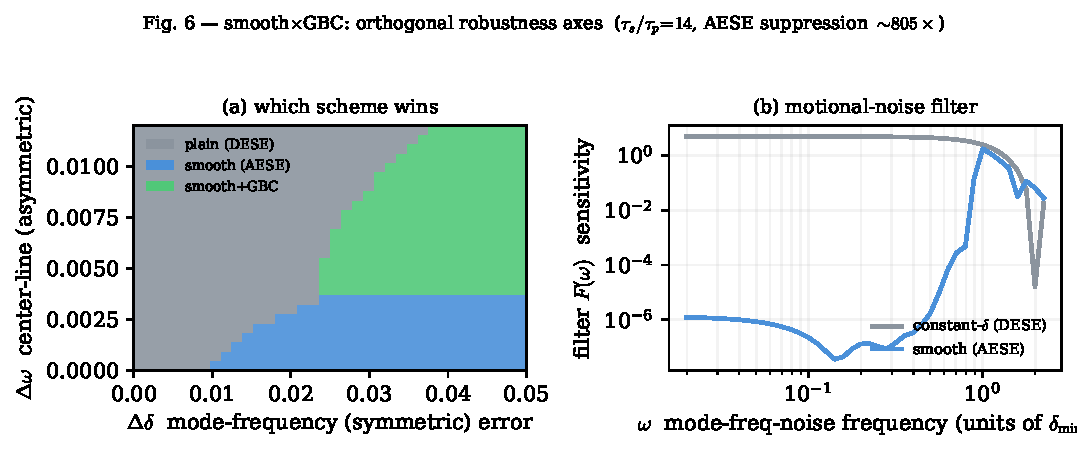
\includegraphics[width=\columnwidth]{Fig6_smooth_gbc}
\caption{E7, smooth gate $\times$ GBC (two orthogonal robustness axes). (a)~Decision map over the
symmetric ($\Delta\delta$) and asymmetric ($\Delta\omega$) error axes at fixed noise: color is the
lowest-infidelity scheme of \{plain, smooth, GBC, smooth+GBC\}. Plain wins near the origin, smooth
(AESE) along the $\Delta\delta$ axis, smooth+GBC in the both-large corner; pure GBC never wins in
range. (b)~Motional-noise filter $F(\omega)$: the smooth (AESE) gate is $\sim\!10^{6}\times$ below
the constant-$\delta$ (DESE) gate at low frequency --- the temperature-insensitivity mechanism of
Ref.~\cite{Hughes25}. ($\tau_{\rm smooth}/\tau_{\rm plain}\!\approx\!14$; AESE spin--motion
suppression $\sim\!800\times$ at $\Delta\delta=0.02$.)}\label{fig:e7}\end{figure}

\section{Discussion}\label{sec:disc}
The results establish five points. (i)~The closed-system agreement between an $O(M)$ analytic
engine and a full Lindblad integrator ($|\Delta F|\sim10^{-9}$--$10^{-6}$) makes design cheap
and verification trustworthy. (ii)~Robust waveforms and GBC trade coherent suppression for
gate~time, so their benefit is conditional on the incoherent budget: below $\Delta\omega^\times$
use the single robust gate, above it use GBC. (iii)~The useful robustness depth is shallow
($k^\star\!\in\!\{0,1\}$); over-compensating is strictly counterproductive. (iv)~The trade-off
survives in a real chain (target-mode-dominated incoherent sensitivity). (v)~Robustness has
\emph{two orthogonal axes}, and the framework's second use is deciding when to \emph{combine}
techniques: the smooth gate (AESE) is the strongest symmetric-axis tool but, being $\sim\!14\times$
longer, the most exposed on the asymmetric axis, so appending GBC pays above
$\Delta\omega^\times\!\approx\!3.5\times10^{-3}$ --- and, tellingly, pure GBC never wins in the
mapped window, because whenever $\Delta\omega$ is large enough to need it the symmetric axis already
calls for the smooth gate (E7). This is the same coherent--incoherent logic as (ii), now on a
$(\Delta\delta,\Delta\omega)$ plane. The framework is
agnostic to the pulse-design method: since $\Delta\omega^\times$ depends on a scheme only
through $I_{\rm incoh}\!\propto\!\tau$, any robust waveform closing the same modes in comparable
time lands at the same crossover, as E6 confirms directly.

\emph{Experimental considerations.} The waveform is piecewise-constant with $4M+4$ segments;
for $M=3$ over $\tau\sim100~\mu$s this is a $\sim\!160$~kHz amplitude-update rate, within
standard AWG/DDS control of an AOM. The AM peak Rabi frequency exceeds the constant-closure
value by $\sim\!4\times$; the PM variant removes this. Calibration uses the same inputs as a
standard MS gate (mode frequencies, $\eta$, one global Rabi scale). Pulse-timing jitter is a
distinct axis, quantified directly (\textsf{ion-jitter}): a common/systematic timing offset is
strongly suppressed ($\sim\!30\times$), but independent per-boundary jitter is \emph{not}
self-cancelled --- it degrades fidelity $\propto\sigma_t^2$ and scales with the segment count, so
a shaped robust waveform carries a genuine timing-jitter cost that a constant-amplitude gate (no
interior boundaries) does not.

\emph{Limitations.} The analytic operator is second-order Magnus~\cite{Zhang25}. The
open-system verifier's Hilbert space grows as $4\prod_m N_{\rm Fock}^{(m)}$, run here at
$M\!\le\!3$ ($\dim=640$); this is \emph{not} a $2^N$ wall (a pairwise gate is two qubits
$\otimes$ its coupled modes). Three routes extend it: E5-justified reduced-mode models (a
spectator's weight falls with detuning, a computable error bar), quantum-trajectory
unravelling ($\dim$ statevectors, already implemented in \textsf{ion-ms-exact}), and adiabatic
elimination or a $\kappa\tau$ cumulant expansion ($O(\dim)$). The noise model is Markovian with
constant rates --- appropriate for the incoherent floor and for white dephasing, but not for
$1/f$/correlated heating; note that the two limiting timescales (quasi-static coherent drift,
targeted by the robust waveform, and white incoherent noise) are both modeled, and the
$\sqrt{I_{\rm incoh}}$ structure is generic to any positive-weight spectrum. Single-qubit gates
in GBC are taken ideal (or SUPCODE-protected) as in Ref.~\cite{Zhang25}.

\section{Conclusion}
We built a design$\to$open-system-verify toolchain for robust MS gates and used it to quantify
the coherent--incoherent trade-off that governs whether robust-control gains survive
dissipation. The headline is a map: robustness pays off only above a noise-set threshold
$\Delta\omega^\times\!\propto\!\sqrt{I_{\rm incoh}}$, and the useful compensation depth is
$k^\star\!\in\!\{0,1\}$ --- one GBC or none. These conclusions are species-independent in
dimensionless units, robust to spectator-mode load, and validated against a full non-RWA +
beyond-Lamb-Dicke model. Bringing the smooth gate (AESE) into the same framework extends the picture
to a \emph{second robustness axis}: symmetric- and asymmetric-axis robustness are orthogonal and
additive, so the practical question becomes \emph{when to combine} them --- a four-scheme decision
map with an add-GBC threshold $\Delta\omega^\times\!\approx\!3.5\times10^{-3}$, in which smooth+GBC
wins only when both error axes are large. Together these give a pre-hardware calibration rule for
MS gates at $2$--$4$ ions.

\begin{acknowledgments}
CiRA QuantumSim (KMITL). Software cross-validated against the analytic framework
of~\cite{Zhang25}.
\end{acknowledgments}

\appendix

\section{Notation map (paper $\leftrightarrow$ code)}\label{app:notation}
{\scriptsize
\begin{ruledtabular}
\begin{tabular}{@{}p{0.27\columnwidth}p{0.24\columnwidth}p{0.33\columnwidth}@{}}
quantity & symbol & module:function \\ \hline
entangling phase & $\Theta(\tau)$ & \textsf{shapedThetaEnt} \\
mode displacement & $\alpha_m(\tau)$ & \textsf{envelope} \\
closure residual & $|\alpha_m(\tau)|$ & \textsf{shapedResiduals} \\
robust waveform & $A\mathbf x{=}0$, $\mathbf x^{\mathsf T}\!M\mathbf x{=}\Xi$ & \textsf{solveShapeRobust} \\
asymmetric err.\ / GBC & $\Delta\omega$, $\hat K_{\mathcal G}$ & \textsf{ion-gbc:gbcUnitaryK} \\
mode spectrum & $\{\omega_m,b^m_j\}$ & \textsf{ion-modes} \\
open-system evolution & Lindblad $\dot\rho$ & \textsf{ion-ms}, \textsf{ion-ms-mm} \\
non-RWA / beyond-LD & $\sin[\eta(a{+}a^\dagger)]$ & \textsf{ion-ms-exact} \\
smooth-gate displ. & $\dot\alpha{=}{-}i(\delta\alpha{+}\Omega)$ & \textsf{ion-smooth:integrateAlpha} \\
adiabatic ramp & $\delta(s){=}(b{+}cg)^{-1/j}$ & \textsf{ion-smooth:smoothProtocol} \\
motional-noise filter & $F(\omega)$ & \textsf{ion-smooth:filterFunction} \\
smooth$\times$GBC map & $1{-}F(\Delta\delta,\Delta\omega)$ & \textsf{ion-smooth:schemes} \\
\end{tabular}
\end{ruledtabular}
}

\section{The center-line error $\varepsilon\equiv\Delta\omega\tau$ and the $\varepsilon^2\!\to\!\varepsilon^4$ scaling}\label{app:eps}
The trade-off is organized by the dimensionless \emph{center-line error}
$\varepsilon\equiv\Delta\omega\,\tau$: the total unwanted rotation the gate accumulates.
$\Delta\omega$ is the asymmetric (center-line) drift --- a common $\sigma_z$ rotation on both
qubits at rate $\Delta\omega$ --- and $\tau$ is the gate time, so $\varepsilon$ is that rate
integrated over the gate, in radians. It is small ($\varepsilon\ll1$) in any working device,
which licenses the expansion. (A $\delta=2\pi\times50$~kHz gate has $\tau\approx20~\mu$s, so a
drift $\Delta\omega=2\pi\times0.4$~kHz gives $\varepsilon\approx0.05$.)

From Eq.~\eqref{eq:star} the imperfect gate is $\hat U_\varepsilon=\hat U_{\rm ideal}\exp(-i\varepsilon E)$,
$E=\tfrac12\sum_j\sigma_z^j$. The symbol ``$\varepsilon^2\!\to\!\varepsilon^4$'' is how the
\emph{infidelity} $1-F$ scales, uncompensated versus with GBC. Uncompensated, a small over-rotation
by $\varepsilon$ has $F\simeq\cos^2(\varepsilon/2)$, so $1-F\simeq(\varepsilon/2)^2\propto\varepsilon^2$
(error amplitude $O(\varepsilon)$). GBC's three-gate echo cancels the first-order-in-$\varepsilon$
term exactly, leaving amplitude $O(\varepsilon^2)$; as infidelity is amplitude squared,
$1-F\propto\varepsilon^4$. Literally: doubling $\varepsilon$ raises the single-gate error $4\times$
($=2^2$) and the GBC error $16\times$ ($=2^4$) (measured $3.99$, $15.95$). Since $\varepsilon<1$,
$\varepsilon^4\!\ll\!\varepsilon^2$:

The columns below are the infidelity $1{-}F$ (single gate and GBC):
\begin{ruledtabular}\begin{tabular}{cccc}
$\varepsilon{=}\Delta\omega\tau$ & single $\propto\varepsilon^2$ & GBC $\propto\varepsilon^4$ & suppression \\ \hline
$0.02$ & $1.3\times10^{-4}$ & $1.4\times10^{-8}$ & $9.5\times10^{3}$ \\
$0.05$ & $8.1\times10^{-4}$ & $5.4\times10^{-7}$ & $1.5\times10^{3}$ \\
$0.10$ & $3.2\times10^{-3}$ & $8.5\times10^{-6}$ & $3.8\times10^{2}$ \\
$0.20$ & $1.3\times10^{-2}$ & $1.3\times10^{-4}$ & $95$ \\
\end{tabular}\end{ruledtabular}

This $\varepsilon^4$ gain costs the GBC sequence's $4\tau$ duration ($\approx4\times$ incoherent
error), so GBC pays off only where $\varepsilon$ is large enough that removing the $\varepsilon^2$
coherent error outweighs the $4\times$ incoherent cost --- the crossover $\Delta\omega^\times$ (E2--E3).

\section{The smooth gate (AESE): semiclassical model and combining logic}\label{app:smooth}
In the forced ($\pm$) spin sector the single-mode MS interaction is
$\hat H=\delta(t)a^\dagger a+\Omega(t)(a+a^\dagger)$, so the coherent displacement
$\alpha(t)=\langle a\rangle$ obeys Eq.~\eqref{eq:aese}, $\dot\alpha=-i(\delta(t)\alpha+\Omega(t))$,
$\dot\theta_g=\Omega^2/\delta$; the gate is Bell-making at $\alpha(\tau)=0$, $\theta_g=\pi/2$.
\textsf{integrateAlpha} propagates this by RK4 (one complex number, no Fock space), exact for the
coherent diagnostics. Two closures: \emph{DESE} ($\delta$ const, fast $\Omega$) traces a circle of
radius $\Omega/\delta$, closing at $\tau=2\pi K/\delta$, with residual \emph{linear} in a static
$\Delta\delta$; \emph{AESE} ($\Omega\approx$ const, $\delta(s)=(b+c\,g(s))^{-1/j}$ swept slowly,
\cite{Hughes25} Eq.~18) tracks $-\Omega/\delta(t)$ and returns to the origin via $\Omega\!\to\!0$
independently of $\Delta\delta$ (residual suppressed $\sim\!800\times$ at $\Delta\delta=0.02$). The
filter function $F(\omega)=\langle|\alpha(\tau)|^2\rangle_\varphi/\varepsilon^2$ for
$\delta\!\to\!\delta+\varepsilon\cos(\omega t+\varphi)$ (\textsf{filterFunction}, averaged over
$\varphi\in\{0,\pi/2\}$) is $\sim\!10^{6}\times$ below DESE at low $\omega$ (Fig.~\ref{fig:e7}b).
The combining model scores scheme $\in\{$plain, smooth, gbc, smoothGbc$\}$ as
$1{-}F=(2\bar n{+}1)|\alpha_{\rm res}(\Delta\delta)|^2+c(\Delta\omega\tau)+[\kappa\int|\alpha|^2(2\bar n{+}1)+\gamma_\phi\tau]\times\{1\text{ or }4\}$,
with $|\alpha_{\rm res}|$ the DESE or AESE static-drift residual, $c(\varepsilon)$ the U2 coherent
term ($\varepsilon^2$ / $\varepsilon^4$), $\tau\in\{\tau_{\rm plain},\tau_{\rm smooth}\}$, and the
$\times4$ for the GBC variants ($4\tau$). \textsf{schemes} evaluates all four, \textsf{winner}
returns the minimum, and \textsf{crossoverDeltaOmega} locates $\Delta\omega^\times$. This is a
leading-order model (so labelled in the code): it neglects cross-terms between the two coherent axes
and between coherent and incoherent errors --- each a product of independently small quantities ---
the same additive-decomposition premise validated for the single-axis trade-off in E1--E3.

\bibliographystyle{apsrev4-2}
\bibliography{references}

\end{document}
